\subsection{Import View Points}
\label{sec:ui_import_viewpoints}

This task allows importing of view points and respective ASTERIX data recording files into the opened database. \\

%TODO_V7

\begin{figure}[H]
  \center
    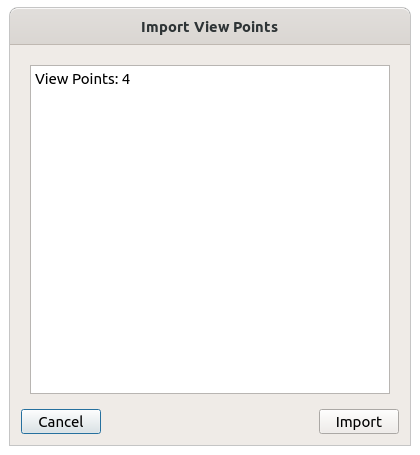
\includegraphics[width=8cm]{figures/view_point_import.png}
  \caption{Import View Points}
\end{figure}

After selection of a view point file, a text field is given which, displays the view point context information or an error message. \\

At the bottom, an 'Import' button exist, which is only enabled if a valid file was selected.

\subsubsection{Notes}

For a detailed specification of a view point file, please refer to \nameref{sec:appendix_view_points}. \\

For each of the datasets, an 'Import ASTERIX Recording' task is started, in the configuration that was set previously. Please make sure that the configuration is valid for such processing. \\

For the filename in each dataset, the absolute path is searched first. If such a file can not be found, a file with the same name but in the location of the view point file is searched also. If the referred file can not be found, an error message is displayed. \\

It is not recommended to import multiple view point files, such a use case is not yet fully supported.

Using the 'Import' button a process is started to import the view points and ASTERIX data recordings. \\

